\documentclass[UTF-8, 10pt]{ctexart}
    \usepackage{geometry}
    \usepackage{fancyhdr}
    \usepackage{enumerate}
    \usepackage{graphicx}
    \usepackage{subfigure}
    \usepackage{titlesec}
    \usepackage{float}
    \usepackage{amsmath, amssymb}
    \usepackage{parskip}
    \usepackage{array}
    \usepackage{listings}
    \usepackage{xcolor}
    \usepackage{fontspec}
    \usepackage{indentfirst}
    \usepackage{makecell}
    \usepackage[breaklinks,colorlinks,linkcolor=black,citecolor=black,urlcolor=black]{hyperref}
    \pagestyle{fancy}
    \lhead{}
    \chead{}
    \rhead{}
    \lfoot{}
    \cfoot{\thepage}
    \rfoot{}
    \renewcommand{\headrulewidth}{0pt}
    \addtolength{\parskip}{-.5em}
    %\CTEXsetup[name={,、},number={\chinese{section}},format={\Large\bfseries}]{section}
    \titleformat{\section}{\bfseries\Large}{\chinese{section}、}{.5em}{}
    \titleformat{\subsection}{\bfseries\large}{(\chinese{subsection})}{.5em}{}
    \titleformat{\subsubsection}{\bfseries}{\arabic{subsubsection}}{.5em}{}
    \titlespacing{\section}{0em}{*1.5}{*1.1}
    \titlespacing{\subsection}{1em}{*1.5}{*1.1}
    \titlespacing{\subsubsection}{2em}{*1.5}{*1.1}
    \setlength{\parindent}{2em}
    
    \lstset{
        columns=fixed,       
        numbers=left,                               % 在左侧显示行号
        numberstyle=\tiny\color{gray},                    % 设定行号格式
        frame=none,                                 % 不显示背景边框
        backgroundcolor=\color[RGB]{245,245,244},         % 设定背景颜色
        keywordstyle=\color[RGB]{40,40,255},              % 设定关键字颜色
        numberstyle=\footnotesize\color{darkgray},           
        commentstyle=\color{gray},             % 设置代码注释的格式
        stringstyle=\rmfamily\slshape\color[RGB]{128,0,0},   % 设置字符串格式
        showstringspaces=false,                        % 不显示字符串中的空格
        %language=c++,                               % 设置语言
    }
    
    
    %\includegraphics{*.png}
    \geometry{left = 3cm, right = 3cm, top = 3cm, bottom = 3cm}
    \title{数据科学导论大作业报告-LMP短期预测}
    \author{王铮澄\ 林啸\ 牛腾腾}
    \date{\today}
    \begin{document}
        \maketitle
            \section{选题意义}
                \indent{}节点边际电价(Locational marginal price)是一种基于最优潮流的电价算法,这种方式得到的节点电价
                会受到4个因素影响:发电机边际成本,系统容量,网损和线路阻塞情况。而节点电价电力市场在国外已经有多年的发展和使用历史。
                不同于我国电力市场统一定价的方式,在基于节点电价的电力市场中,每个节点的电价都可能不相同,受到上述4个因素影响。
                一般来说,当线路出现阻塞或是某区域电力负荷较高时,节点电价会被抬高。
                典型的使用节点电价的电力市场:美国PJM电力市场、加州电力市场CAISO、澳洲电力市场、欧洲电力市场。
                我国即将在广东试行节点电价电力市场,若能准确预测次日LMP,发电商、售电商就能调整竞价策略,获取更高的利润,有其实用意义。
                此外,对节点电价的预测本质上是对时间序列的预测,可以在这个项目中很好地结合本课程所学。\\
            
            \section{项目目标}我们的预测目标是基于历史数据,对次日24小时每小时的日前市场节点电价进行预测。
            在前期文献调研中,国外对于节点电价预测的准确度在MAPE误差之下大都在为10\%左右,并且对尖峰点的预测效果普遍不好,
            因此我们将这次大作业的目标定为预测MAPE误差在12\%以内,并且通过图像来判断尖峰点的预测效果,尽量优化尖峰点处的预测精度。\\
            
            \section{数据分析}
                \indent{}项目数据来源是美国PJM市场官网(www.dataminer2.pjm.com),在前期数据分析中,发现这个网站的数据种类较多,但是
                数据质量参差不齐,而且数据格式并不统一,例如每日发电容量、每小时负荷测量数据等更新不及时,最新的数据一般是几天甚至几个月之前的,
                这对于我们需要的次日预测目标来说是不合用的,因此在选取训练数据的时候需要对数据的实时性加以分析。此外网站上数据的组织形式
                不统一,电价类数据是根据时间和节点进行划分的,每个节点会给出24小时的电价,而负荷类数据是根据区域划分的,并不精确到节点,发电类数据
                则是根据能源种类和更大的区域来划分的,因此都需要专门处理,得到可以训练的向量形式。\\

            \section{符号说明}
            \begin{table}[H]
                \centering
                \begin{tabular}{|c|c|}
                    \hline
                    \makecell{符号} & \makecell{含义}\\ 
                    \hline
                    $load^{t}_{f}$ & 预测日当天时间t的负荷\\
                    \hline
                    $lmp^{t}_{f-n}$ & 预测日前n天时间t的总电价\\
                    \hline
                    $cop^{t}_{f-n}$ & 预测日前n天时间t的电价拥堵分量\\
                    \hline
                    $mlp^{t}_{f-n}$ & 预测日前n天时间t的电价线损分量\\
                    \hline
                    $t$ & 时间t标记,取值为1到24之间的整数\\
                    \hline
                    $spike\_mark^{t}_{f}$ & 预测日时间t的电价尖峰标记,非尖峰为0\\
                    \hline
                    \end{tabular}
            \end{table}
            
            \section{第一阶段}
            \subsection{特征选择与误差评估}
                \indent{}[$load^{t}_{f}$、$lmp^{t}_{f-1}$、$lmp^{t}_{f-2}$、$lmp^{t}_{f-7}$、$t$] 
                共5个特征,在尖峰优化设想当中加入了‘尖峰电价标记’特征。\\
                \indent{}误差函数的选择为MAPE。\\

            \subsection{数据选取与划分}
                \indent{}本次选择的数据为美国PJM电力市场5021071号节点的daily ahead lmp数据,时间跨度为2018.7.2---2018.10.1,
                其中选择7月2日到9月17日的数据作为训练集,9月18日到10月1日的数据作为测试集。\\
            \subsection{模型评估}
                \subsubsection{MLP}
                    \indent{}MLP模型的准确率不是特别稳定,在参数固定的情况下每次运行得到的准确度有1\%左右的波动。\\
                    \indent{}基本参数为:\\
                    \begin{table}[H]
                        \centering
                        \begin{tabular}{|c|c|}
                            \hline
                            \makecell{参数类型} & \makecell{参数详情}\\ 
                            \hline
                            隐层数量 & 2\\
                            \hline
                            隐层节点 & (100,80)\\
                            \hline
                            激活函数 & ‘relu’\\
                            \hline
                            迭代次数 & 50000\\
                            \hline
                            学习率 & 0.1\\
                            \hline
                            优化器 & ‘Adam’\\
                            \hline
                            \end{tabular}
                    \end{table}

                    \indent{}以下为连续三次运行得到的训练集误差率和测试集误差率:\\
                    \begin{table}[H]
                        \centering
                        \begin{tabular}{|c|c|}
                            \hline
                            \makecell{训练集误差/\%} & \makecell{测试集误差/\%}\\ 
                            \hline
                            6.13 & 13.01\\
                            \hline
                            6.36 & 12.42\\
                            \hline
                            6.06 & 13.75\\
                            \hline
                            \end{tabular}
                    \end{table}

                    \indent{}预测图像为:\\
                    \begin{figure}[H]                                        %[htbp]是自动排版     
                        \centering                                                      %图片居中
                        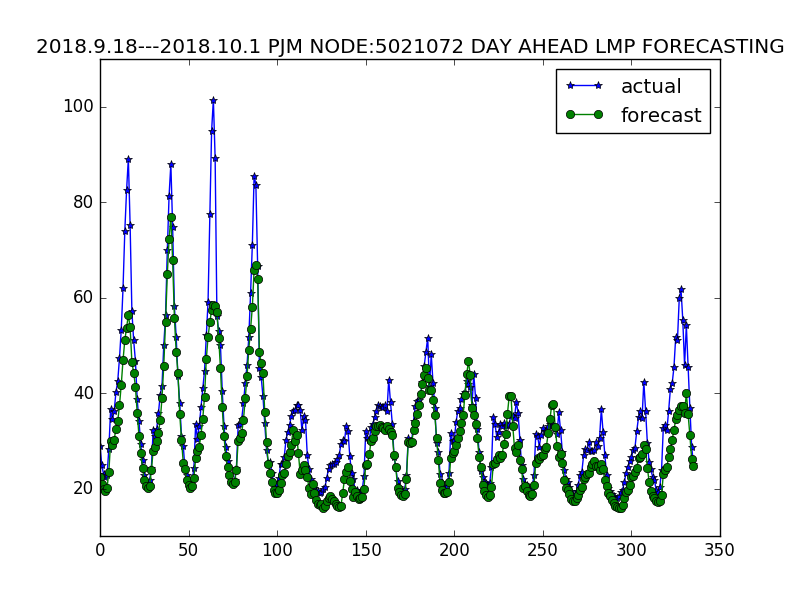
\includegraphics[width = .8\textwidth]{MLP.png}            %设置大小和名称
                        \caption{MLP预测}\label{1}                               %图片名称和图片标号
                        \end{figure}

                \subsubsection{SVM}
                \indent{}基本参数为:\\
                \begin{table}[H]
                    \centering
                    \begin{tabular}{|c|c|}
                        \hline
                        \makecell{参数类型} & \makecell{参数详情}\\ 
                        \hline
                        C & 0.1\\
                        \hline
                        gamma & 0.01\\
                        \hline
                        核函数 & ‘rbf’\\
                        \hline
                        \end{tabular}
                \end{table}

                \indent{}误差率稳定\\
                \begin{table}[H]
                    \centering
                    \begin{tabular}{|c|c|}
                        \hline
                        \makecell{训练集误差/\%} & \makecell{测试集误差/\%}\\ 
                        \hline
                        7.44 & 11.93\\
                        \hline
                        \end{tabular}
                \end{table}

                \indent{}预测图像为:\\
                \begin{figure}[H]                                        %[htbp]是自动排版     
                    \centering                                                      %图片居中
                    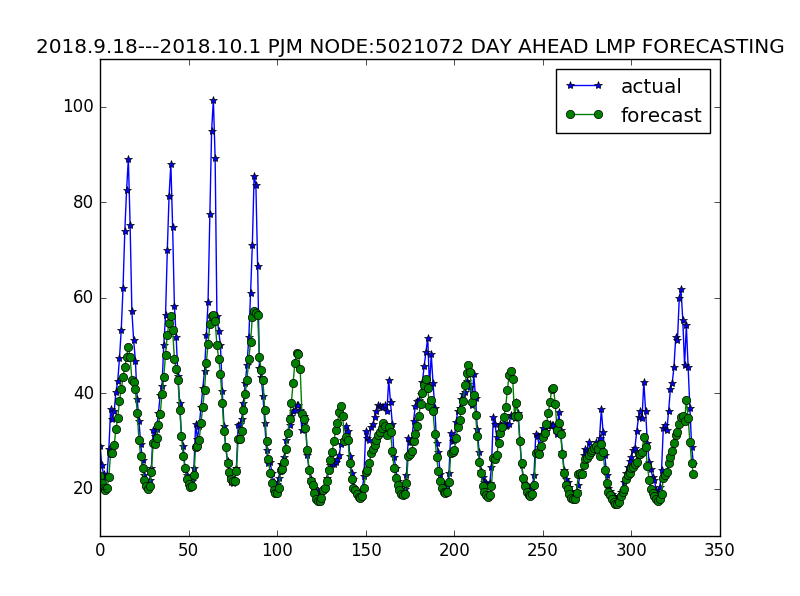
\includegraphics[width = .8\textwidth]{SVM.png}            %设置大小和名称
                    \caption{SVM预测}\label{1}                               %图片名称和图片标号
                    \end{figure}

                \subsubsection{RF}
                \indent{}基本参数为:\\
                \begin{table}[H]
                    \centering
                    \begin{tabular}{|c|c|}
                        \hline
                        \makecell{参数类型} & \makecell{参数详情}\\ 
                        \hline
                        n\_estimators & 60\\
                        \hline
                        max\_depth & 5\\
                        \hline
                        max\_features & 2\\
                        \hline
                        \end{tabular}
                \end{table}

                \indent{}误差率较为稳定,测试集误差波动在0.5\%以内,以下为连续3次训练的误差:\\
                \begin{table}[H]
                    \centering
                    \begin{tabular}{|c|c|}
                        \hline
                        \makecell{训练集误差/\%} & \makecell{测试集误差/\%}\\ 
                        \hline
                        6.45 & 10.23\\
                        \hline
                        6.48 & 10.68\\
                        \hline
                        6.50 & 10.48\\
                        \hline
                        \end{tabular}
                \end{table}

                \indent{}预测图像为:\\
                \begin{figure}[H]                                        %[htbp]是自动排版     
                    \centering                                                      %图片居中
                    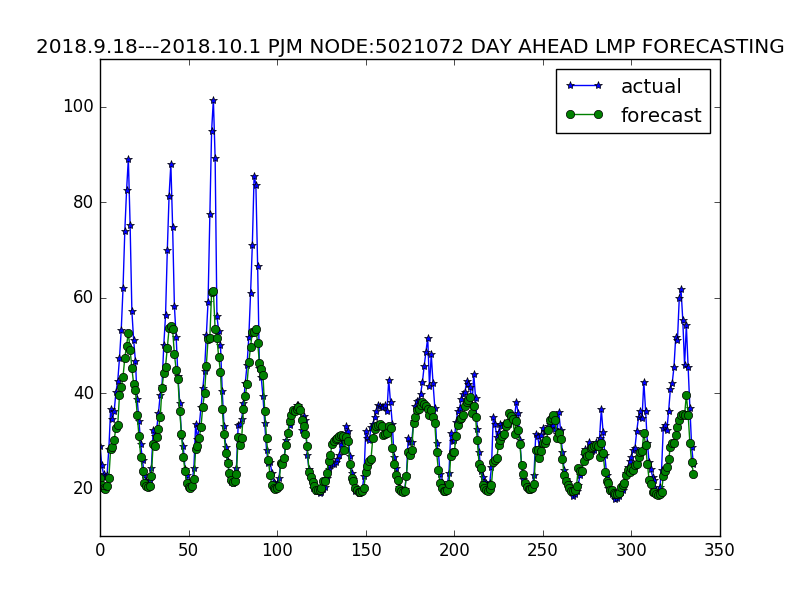
\includegraphics[width = .8\textwidth]{RF.png}            %设置大小和名称
                    \caption{RF预测}\label{1}                               %图片名称和图片标号
                    \end{figure}

                \subsubsection{LGBM}
                \indent{}基本参数为:\\
                \begin{table}[H]
                    \centering
                    \begin{tabular}{|c|c|}
                        \hline
                        \makecell{参数类型} & \makecell{参数详情}\\ 
                        \hline
                        num\_leaves & 4\\
                        \hline
                        max\_depth & 3\\
                        \hline
                        reg\_lambda & 7\\
                        \hline
                        \end{tabular}
                \end{table}

                \indent{}误差率稳定\\
                \begin{table}[H]
                    \centering
                    \begin{tabular}{|c|c|}
                        \hline
                        \makecell{训练集误差/\%} & \makecell{测试集误差/\%}\\ 
                        \hline
                        6.51 & 10.73\\
                        \hline
                        \end{tabular}
                \end{table}

                \indent{}预测图像为:\\
                \begin{figure}[H]                                        %[htbp]是自动排版     
                    \centering                                                      %图片居中
                    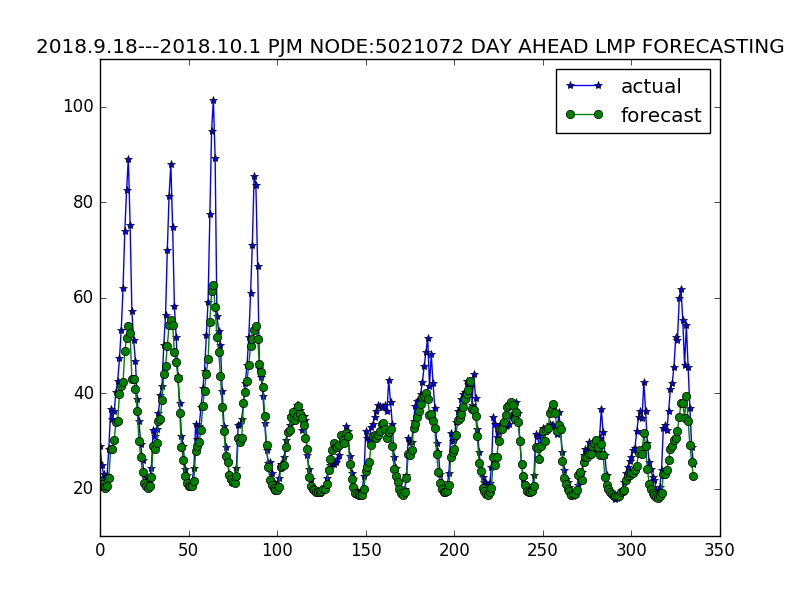
\includegraphics[width = .8\textwidth]{LGBM.png}            %设置大小和名称
                    \caption{LGBM预测}\label{1}                               %图片名称和图片标号
                    \end{figure}

                \subsubsection{XGB}
                \indent{}基本参数为:\\
                \begin{table}[H]
                    \centering
                    \begin{tabular}{|c|c|}
                        \hline
                        \makecell{参数类型} & \makecell{参数详情}\\ 
                        \hline
                        n\_estimators & 150\\
                        \hline
                        max\_depth & 2\\
                        \hline
                        reg\_lambda & 7\\
                        \hline
                        gamma & 0.01\\
                        \hline
                        colsample\_bytree & 0.4\\
                        \hline
                        subsample & 0.6\\
                        \hline
                        learning\_rate & 0.1\\
                        \hline
                        \end{tabular}
                \end{table}

                \indent{}误差率稳定\\
                \begin{table}[H]
                    \centering
                    \begin{tabular}{|c|c|}
                        \hline
                        \makecell{训练集误差/\%} & \makecell{测试集误差/\%}\\ 
                        \hline
                        6.71 & 10.02\\
                        \hline
                        \end{tabular}
                \end{table}

                \indent{}预测图像为:\\
                \begin{figure}[H]                                        %[htbp]是自动排版     
                    \centering                                                      %图片居中
                    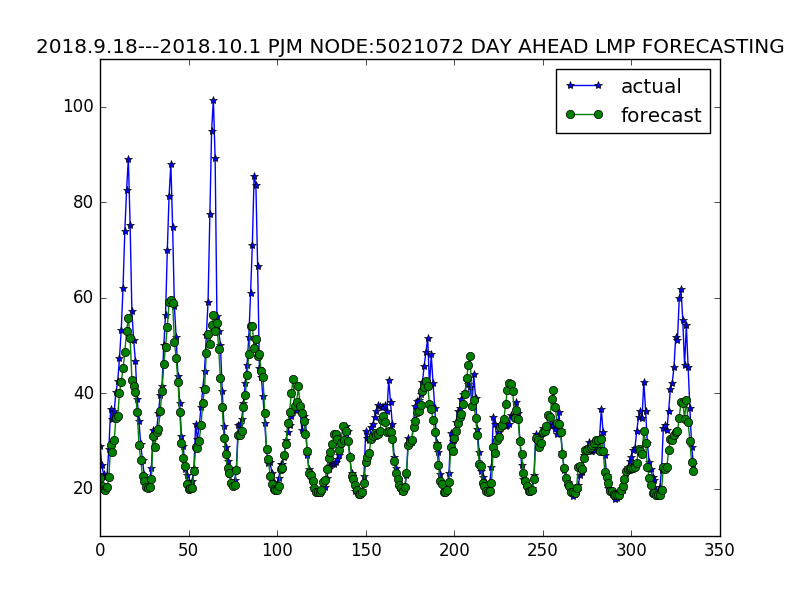
\includegraphics[width = .8\textwidth]{XGB.png}            %设置大小和名称
                    \caption{XGB预测}\label{1}                               %图片名称和图片标号
                    \end{figure}

                \subsubsection{STACK}
                \indent{}将以上五种模型进行stacking,将表现最好的XGB模型作为第二层的回归模型。
                        参数选择与每种模型单独的参数一样。以下列出每种模型单独的MSE Score和其标准差,
                        并将每种模型的训练集、测试集误差汇总。不稳定模型的误差取三次均值。\\

                \begin{table}[H]
                    \centering
                    \begin{tabular}{|c|c|c|c|c|}
                        \hline
                        \makecell{模型名称} & \makecell{MSE Score} & \makecell{标准差} & \makecell{训练集误差/\%} & \makecell{测试集误差/\%}\\ 
                        \hline
                        XGB & -12.25 & +/- 0.0702 & 6.71 & 10.02\\
                        \hline
                        RF & -13.43 & +/- 0.0751 & 6.48 & 10.46\\
                        \hline
                        LGBM & -13.60 & +/- 0.0891 & 6.51 & 10.73\\
                        \hline
                        SVM & -15.18 & +/- 0.0861 & 7.44 & 11.93\\
                        \hline
                        MLP & -13.04 & +/- 0.0839 & 6.18 & 13.06\\
                        \hline
                        STACK & -12.28 & +/- 0.0787 & 5.58 & 11.08\\
                        \hline
                        \end{tabular}
                \end{table}

                \indent{}预测图像为:\\
                \begin{figure}[H]                                        %[htbp]是自动排版     
                    \centering                                                      %图片居中
                    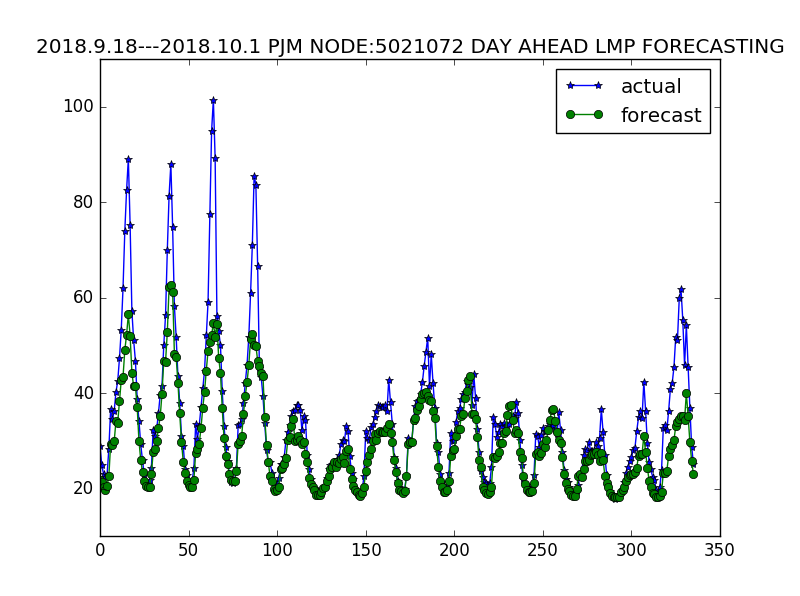
\includegraphics[width = .8\textwidth]{STACK.png}            %设置大小和名称
                    \caption{STACK预测}\label{1}                               %图片名称和图片标号
                    \end{figure}

            \subsection{尖峰优化}
                \indent{}观察到以上模型得到的图像中,对于尖峰点的预测普遍不理想,因此我考虑加入其它特征尝试优化尖峰处的预测。
                    我将训练集中的电价进行分段,先计算出训练集电价的均值$p$和标准差$\delta$,然后以$p$+$\delta$、$p$+1.5$\delta$、
                    $p$+2.5$\delta$作为分界点将电价分为三个等级,分别标记为0,1,2,3。而对于测试集,由于电价事先未知,
                    但是根据预测结果可以看出趋势大致是准确的,所以我考虑先进行第一次训练,然后将预测结果重复对训练集的操作,
                    给预测的电价也进行标号,然后将得到的标号作为特征再次训练,也就是说,在第二次训练的时候我们才将标号作为新特征加入。
                    由于第一次训练之后预测的峰值较小,可能不能被很好地识别和增强,因此我考虑采用多次训练、重标号的办法,使峰值处的电价得以增强。\\
                \indent{}此外,考虑到尖峰电价的形成与线路拥堵状况和损耗状况密切相关,我将这两项也作为特征纳入考虑,在尝试了几种特征组合后,
                    以下的特征表现较好:
                    [$load^{t}_{f}$、$lmp^{t}_{f-1}$、$lmp^{t}_{f-2}$、$lmp^{t}_{f-7}$、$t$、$cop^{t}_{f-1}$、$cop^{t}_{f-7}$、
                    $mlp^{t}_{f-1}$、$mlp^{t}_{f-1}$、$spike\_mark^{t}_{f}$]
                \indent{}由于XGB模型的效果较好,我选择XGB进行尖峰优化。为了对比,XGB模型的参数没有调整。在进行了4轮迭代之后,得到的结果如下:
                \begin{table}[H]
                    \centering
                    \begin{tabular}{|c|c|}
                        \hline
                        \makecell{训练集误差/\%} & \makecell{测试集误差/\%}\\ 
                        \hline
                        5.35 & 8.86\\
                        \hline
                        \end{tabular}
                \end{table}

                \indent{}预测图像为:\\
                \begin{figure}[H]                                        %[htbp]是自动排版     
                    \centering                                                      %图片居中
                    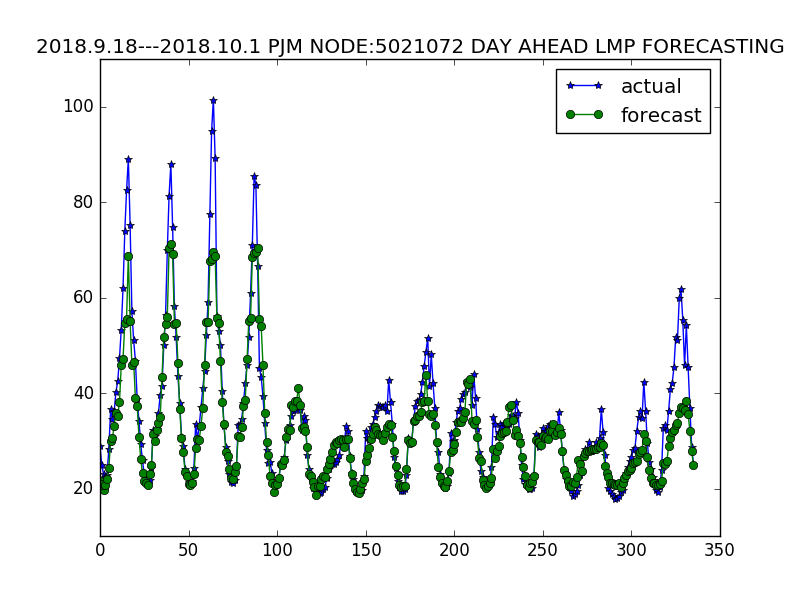
\includegraphics[width = .8\textwidth]{XGB_SPIKE.png}            %设置大小和名称
                    \caption{XGB引入电价标记之后的预测结果}\label{1}                               %图片名称和图片标号
                    \end{figure}

                \begin{figure}[H]                                        %[htbp]是自动排版     
                    \centering                                                      %图片居中
                    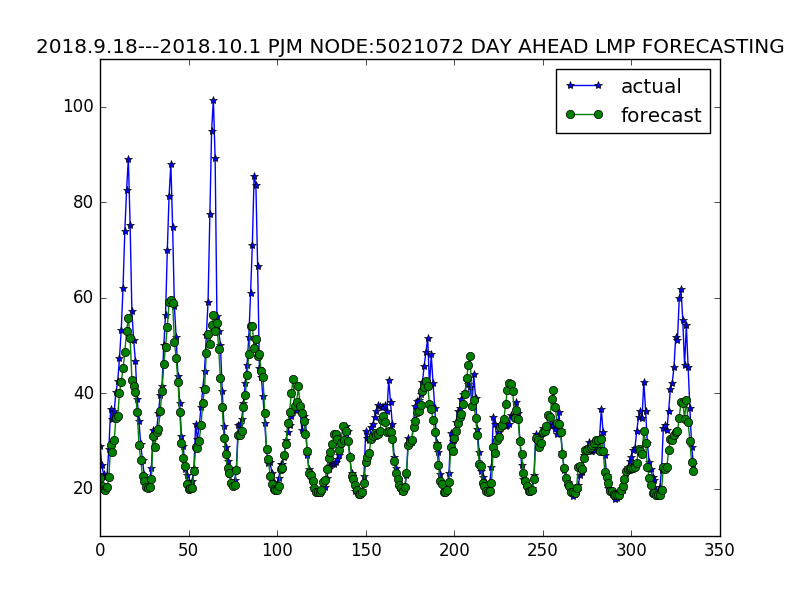
\includegraphics[width = .8\textwidth]{XGB.png}            %设置大小和名称
                    \caption{XGB未引入电价标记的预测结果}\label{1}                               %图片名称和图片标号
                    \end{figure}

                \indent{}从结果可以发现,训练集和测试集上的误差均下降,测试集误差下降大约1.2\%,并且在图像上看出尖峰点有所改善,可以认为
                    该方法确实起到了一定作用。\\
                
            \subsection{结果评估}虽然在调参以及优化之后准确度较高,但是在测试其它节点的时候,我们发现这个模型的效果并不好,误差甚至可以达到
            15\%左右。分析原因,是因为选取的测试数据不够有代表性,这个区间内波形的周期性较为明显,并且几乎没有低洼下陷的波形,
            因此对特征更丰富的数据预测效果较差。因此我们考虑进行第二阶段的探究,使用更多的数据进行训练,测试集也选用更长时间尺度的数据来
            模拟多种情况的预测。\\

            \section{第二阶段}
                \indent{}第二阶段的具体操作步骤与第一阶段大同小异,这里就不再详细描述。具体区别是,我们选用了包括电价分量,负荷,各类能源
                发电量,电力断供量等更多数据,组成了长度为44的特征向量。并且我们使用了接近一年的数据作为训练,两个月的数据进行测试。使用的模型是
                3层MLP。\\
                \indent{}由于数据量较大,特征较多,我使用了自编码器进行主成分分析和特征提取,自编码器的结构设计是4层神经网络,每层以75\%的
                比例缩减。具体见下图:\\
                \begin{figure}[H]                                        %[htbp]是自动排版     
                    \centering                                                      %图片居中
                    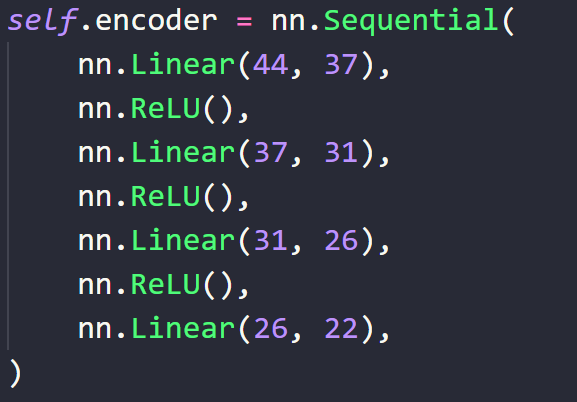
\includegraphics[width = .4\textwidth]{autoencoder.png}            %设置大小和名称
                    \caption{编码器结构}\label{1}                               %图片名称和图片标号
                    \end{figure}

                \subsection{无编码器结果}
                \begin{figure}[H]                                        %[htbp]是自动排版     
                    \centering                                                      %图片居中
                    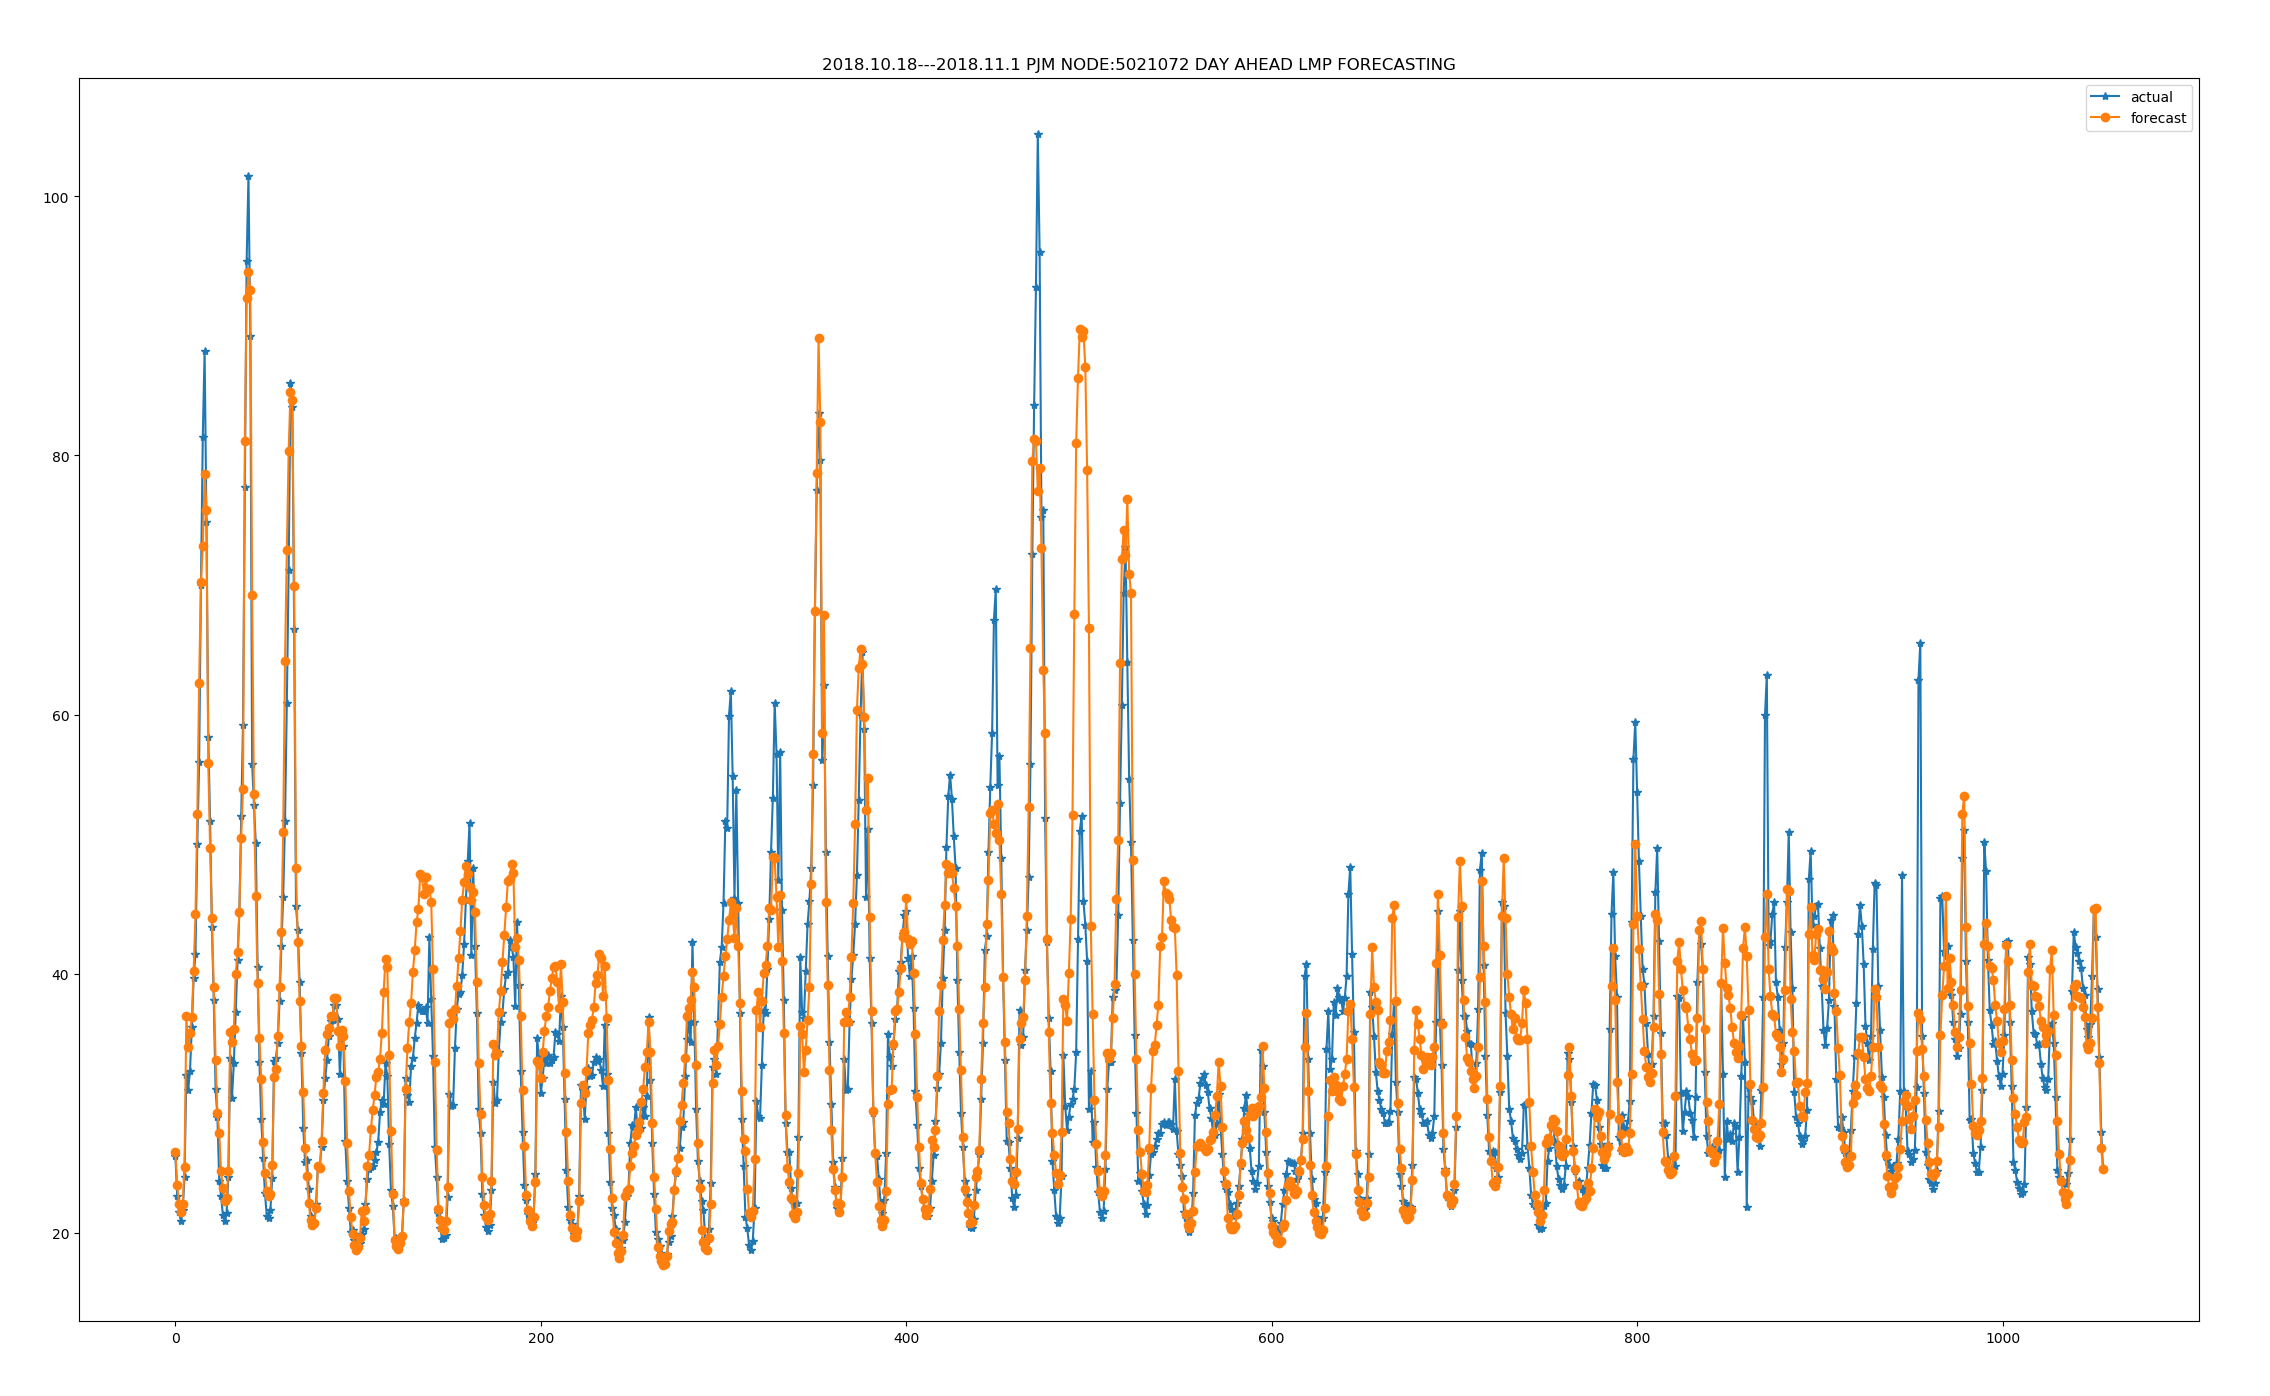
\includegraphics[width = 1\textwidth]{noencoder.png}            %设置大小和名称
                    \caption{无编码器}\label{1}                               %图片名称和图片标号
                    \end{figure}   
                
                \indent{}无编码器时训练误差为3.93\%,测试误差为10.64\%,怀疑有过拟合迹象。\\

                \subsection{有编码器结果}
                \begin{figure}[H]                                        %[htbp]是自动排版     
                    \centering                                                      %图片居中
                    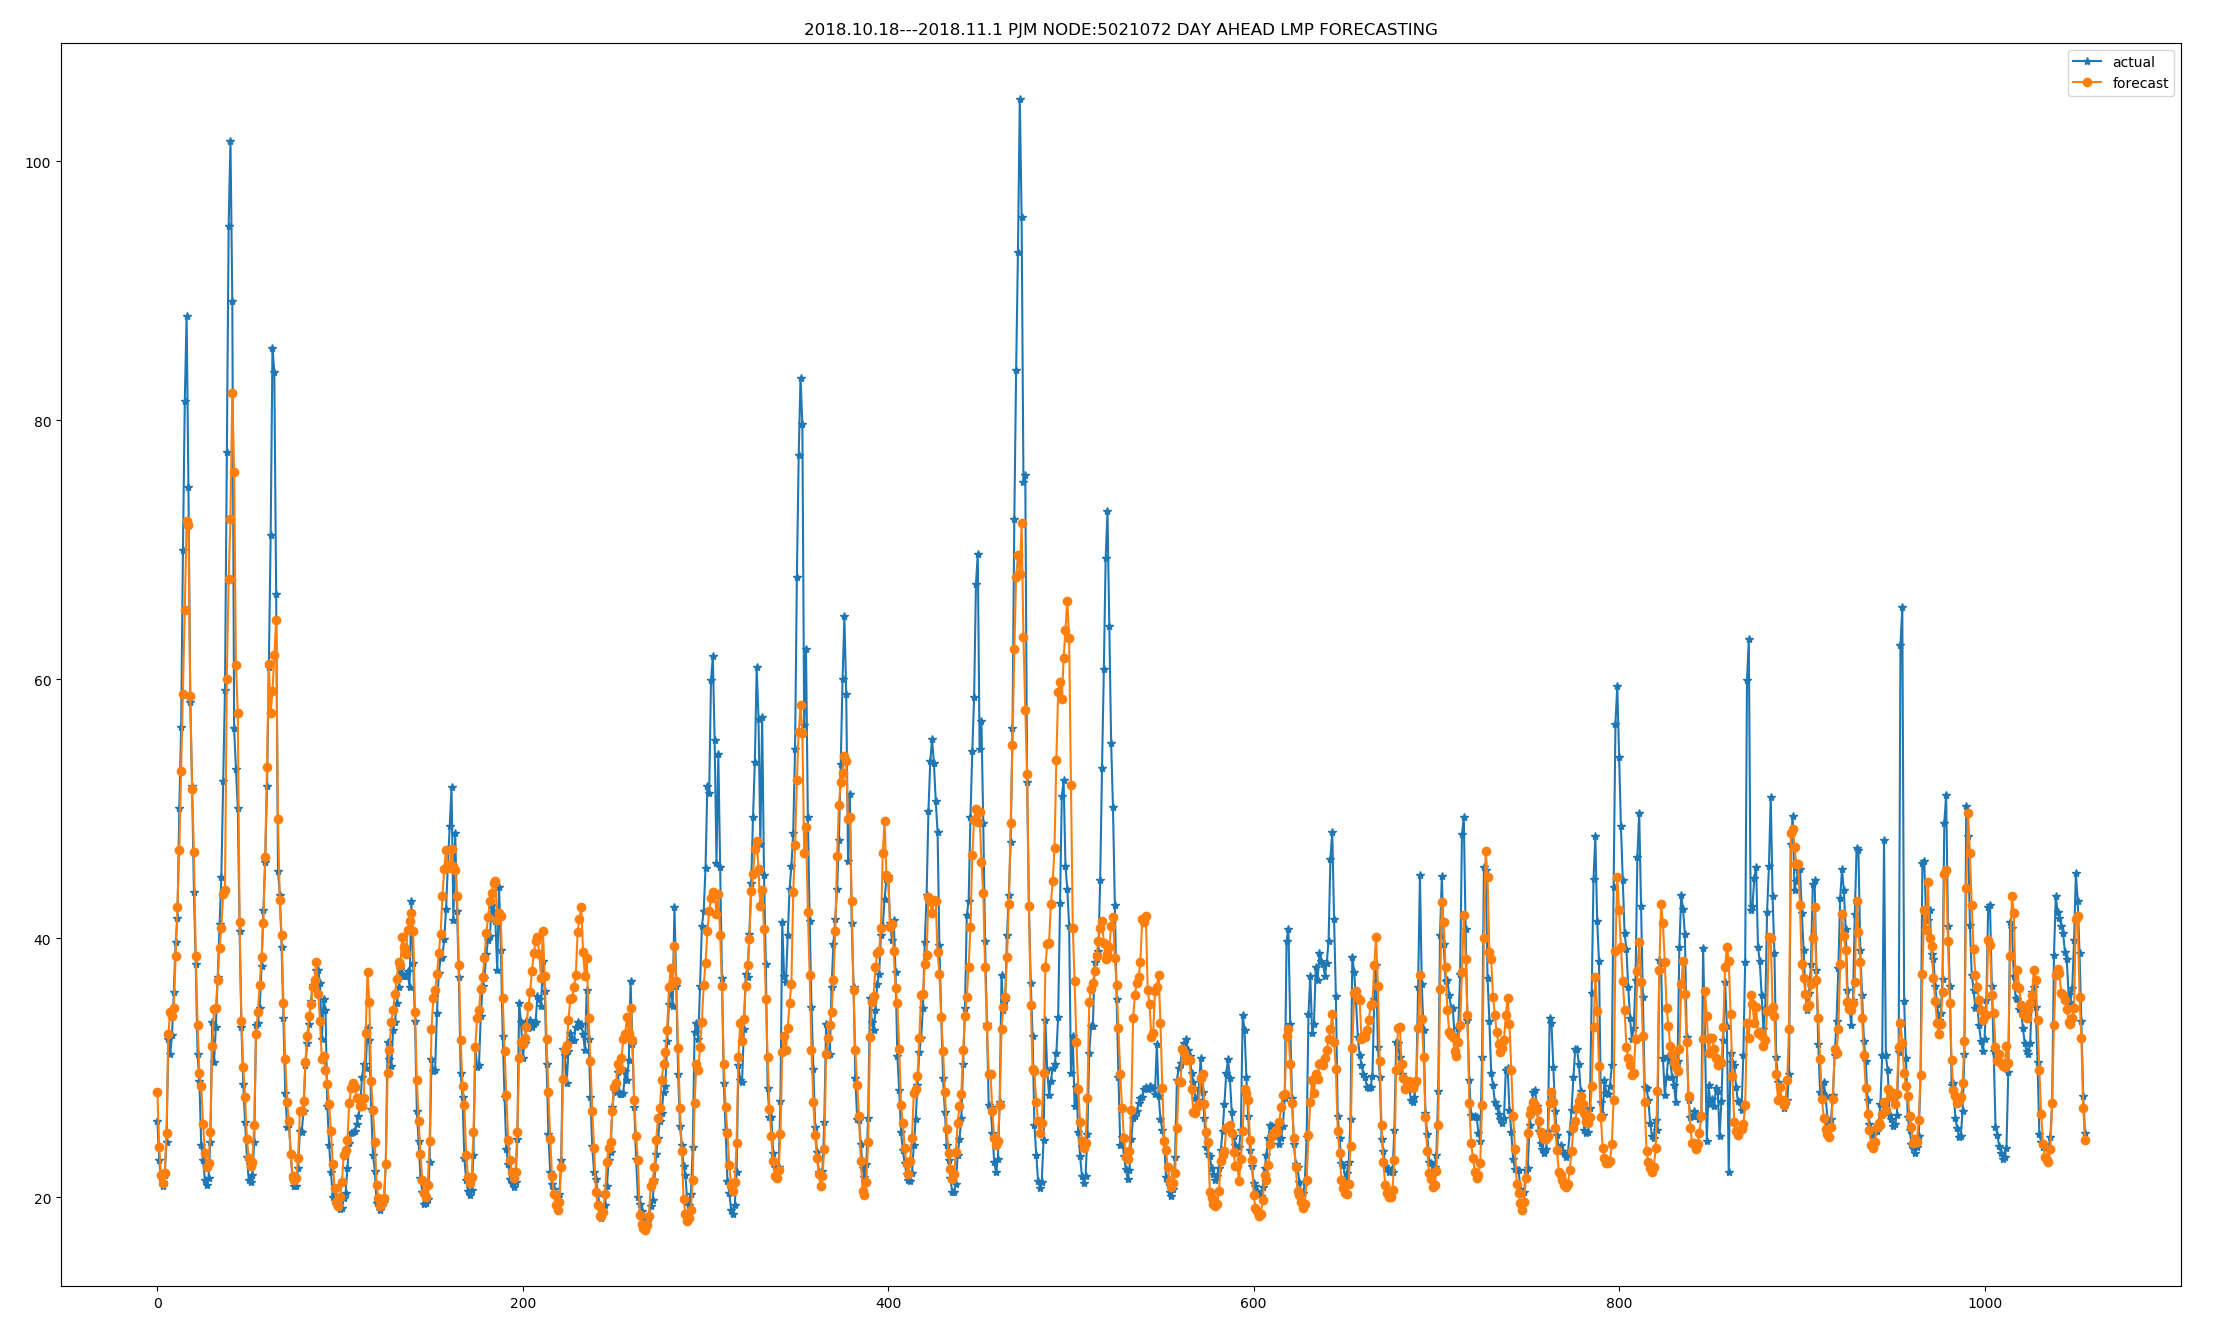
\includegraphics[width = 1\textwidth]{hasencoder.png}            %设置大小和名称
                    \caption{有编码器}\label{1}                               %图片名称和图片标号
                    \end{figure}
                \indent{}有编码器时训练误差为7.03\%,但是测试误差降至10.19\%,训练误差接近测试误差,模型泛化能力变强。\\

                \subsection{结果分析}从误差结果和预测图象上看,数据量加大之后,预测效果明显变好,并且对尖峰点的预测效果大大增强,
                自编码器的使用降低了模型运算量和复杂度,并且提升了模型的泛化能力。预测误差已经达到目标,这次大作业基本得到完成。\\

    \end{document}